\documentclass[a4paper,12pt,oneside]{book}

%-------------------------------Start of the Preable------------------------------------------------
\usepackage[english]{babel}
\usepackage{blindtext}
%packagr for hyperlinks
\usepackage{hyperref}
\hypersetup{
	colorlinks=true,
	linkcolor=blue,
	filecolor=magenta,      
	urlcolor=cyan,
}

\urlstyle{same}
%use of package fancy header
\usepackage{fancyhdr}
\setlength\headheight{26pt}
\fancyhf{}
%\rhead{
\includegraphics[width=1cm]{logo}}
\lhead{\rightmark}
\rhead{
\includegraphics[width=1cm]{logo}}
\fancyfoot[RE, RO]{\thepage}
\fancyfoot[CE, CO]{\href{http://www.e-yantra.org}{www.e-yantra.org}}

\pagestyle{fancy}

%use of package for section title formatting
\usepackage{titlesec}
\titleformat{\chapter}
{\Large\bfseries} % format
{}                % label
{0pt}             % sep
{\huge}           % before-code

%use of package tcolorbox for colorful textbox
\usepackage[most]{tcolorbox}
\tcbset{colback=cyan!5!white,colframe=cyan!75!black,halign title = flush center}

\newtcolorbox{mybox}[1]{colback=cyan!5!white,
	colframe=cyan!75!black,fonttitle=\bfseries,
	title=\textbf{\Large{#1}}}

%use of package marginnote for notes in margin
\usepackage{marginnote}

%use of packgage watermark for pages
%\usepackage{draftwatermark}
%\SetWatermarkText{
\includegraphics{logo}}
\usepackage[scale=2,opacity=0.1,angle=0]{background}
\backgroundsetup{
	contents={
\includegraphics{logo}}
}

%use of newcommand for keywords color
\usepackage{xcolor}
\newcommand{\keyword}[1]{\textcolor{red}{\textbf{#1}}}

%package for inserting pictures
\usepackage{graphicx}

%package for highlighting
\usepackage{color,soul}

%new command for table
\newcommand{\head}[1]{\textnormal{\textbf{#1}}}


%----------------------End of the Preamble---------------------------------------


\begin{document}
	
	%---------------------Title Page------------------------------------------------
	\begin{titlepage}
		\raggedright
		{\Large eYSIP-2017\\[1cm]}
		{\Huge\scshape Development of Web Interface for GH Farm produce \\[.1in]}
		\vfill
		\begin{flushright}
			{\large Hemang Gandhi \\}
			{\large Keivan Shah \\}
			{\large Mentors : Yogita Mali, Uma Sharma, Parin Chedda \\}
			{\large Duration of Internship: $ 22/05/2017-07/07/2017 $ \\}
		\end{flushright}
		
		{\itshape 2017, e-Yantra Publication}
	\end{titlepage}
	%-------------------------------------------------------------------------------
	
	\chapter[Project Tag]{Development of Web Interface for GH Farm produce}
	\section*{Abstract}
	This project is part of the Eyantra Summer Internship Programme 2017. The main aim of this project to make a automated system for the Logging and Monitoring of Farm produce of greenhouses. The system consists of a smart weighing machine powered by Raspberry Pi which logs all the data about the produce such as weight, crop type, trough id, time, etc. The details are then sent to server which maintains all the data and can provide analytics about the data. The smart weighing machine was developed last year as part of eYSIP'16 and the main goal of this years project is to improve the weighing machine, setup a web interface for the data and if possible an e-commerce website to buy and sell the GH farm produce.
	
	\subsection*{Completion status}
	The project is successfully completed. We have successfully created an interface for each of the three users namely producer, consumer and admin providing different functionalities.
	
	\section{Hardware Parts}
	\begin{itemize}
		\item Hardware parts
		\begin{itemize}
			\item Load cell
			\item 20x4 LCD
			\item 4x4 Keypad
			\item Raspberry pi 2 Model B
			\item LM2596 step-down voltage regulator
			\item HX711(ADC amplifier)
			\item USB Camera
			\item DC Adapter
			\item Enclosure to hold all parts
		\end{itemize}
		\item Detail of each hardware:\\
		\href{https://cdn.sparkfun.com/datasheets/Sensors/ForceFlex/hx711_english.pdf}{HX711 ADC Amplifier}\\
		\href{http://www.kadcontrols.com/KadWebsite/LoadCell_Tech/CZL601.pdf}{Load cell CZL601}\\
		\href{http://www.onsemi.com/pub_link/Collateral/LM2596-D.PDF}{Step down voltage regulator}\\
		\href{http://lispol.com/uploaded/products_files/1364491305_79923300.pdf}{20x4 LCD}\\
		\href{https://www.parallax.com/sites/default/files/downloads/27899-4x4-Matrix-Membrane-Keypad-v1.2.p    df}{Membrane Keypad}\\
		\href{https://cdn-shop.adafruit.com/pdfs/raspberrypi2modelb.pdf}{Raspberry pi 2 Model B}\\
		\href{https://www.parallax.com/sites/default/files/downloads/27899-4x4-Matrix-Membrane-Keypad-v1.2.pdf}{4x4 Keypad}\\
		\\
		Hardware is not in the scope of this project
		Please refer last year's \href{https://github.com/Ankurrpanwar26/eYSIP-2016-Farm-Produce-Logging-and-Monitoring/blob/master/Final%20Report/EYSIP_final.pdf}{repository} to get more details about the weighing machine and connections
		\end{itemize}
		
		\section{Software Used}
		\begin{itemize}
			\item Python 3.5.2
			\item Django 1.11.1
			\item Bootstrap 4
			\item HTML 5
		\end{itemize}
		For installation of required softwares refer our \href{https://github.com/eYSIP-2017/eYSIP-2017_Development_of_Web_Interface_for_GH_Farm_Produce/wiki}{wiki} 
		
		\newpage
		
		\section{Software and Code}
		
		\subsection{Smart Weighing Machine}
		The smart weighing machine consists of a Raspberry Pi, LCD display, keypad, load cell and a camera. To log the produce the producer places the produce from the GH farm on the weighing machine. The weighing machine with the help of the the load cell displays the weight on the LCD screen. So the machine can be used as a normal weighing machine. It also has standard weighing machine features like tare. Now the producer can log the produce by pressing * on the keypad. The Raspberry Pi then takes a picture of the produce and sends it to a prediction server to guess the type of the crop. The producer is then shown the possible crops as predicted by the Vegetable Identification using Transfer Learning project. If the crop predicted is correct, the producer can continue or else he can change the crop by selecting one from a list of crops shown sorted according to the confidence of the predicting system or by inputting in the crop id. Once he enters the crop id the enter data is sent to the server for Logging. The data is logged and also made available for selling on the e-commerce website. The data is sent via HTTP requests making use of the modern REST API.
		\subsection{Web Interface}
		The web interface for this project was written in Python using Django. The web interface has mainly three applications, they are:
		\subsubsection{FarmApp:}
		This is the main App of the system. It provides with all the UI that the users i.e. Admin, Producer and Customers interact with.
		\subsubsection{Machine:}
		This app is used only by smart weighing machine to log the produce. The data logged by the machine is sent via HTTP requests to this server for logging. Once the data reaches here it added into the system for buying as well as monitoring.
		\subsubsection{Predict:}
		This is an utility app that runs the Vegetable Identification algorithm on the image sent to it and returns a list of possible crops along with the confidence percentages. This app is used by the smart weighing machine to guess the vegetable by the picture it takes with the webcam attached to it.
		
		\section{Use and Demo}
		\subsubsection{Admin Interface:}
		Admin has control over the entire database and make modifications to the data as and when required. It is his responsibility to add new Producers or Crops into the database.
		\begin{figure}[!ht]
			\centering
			
			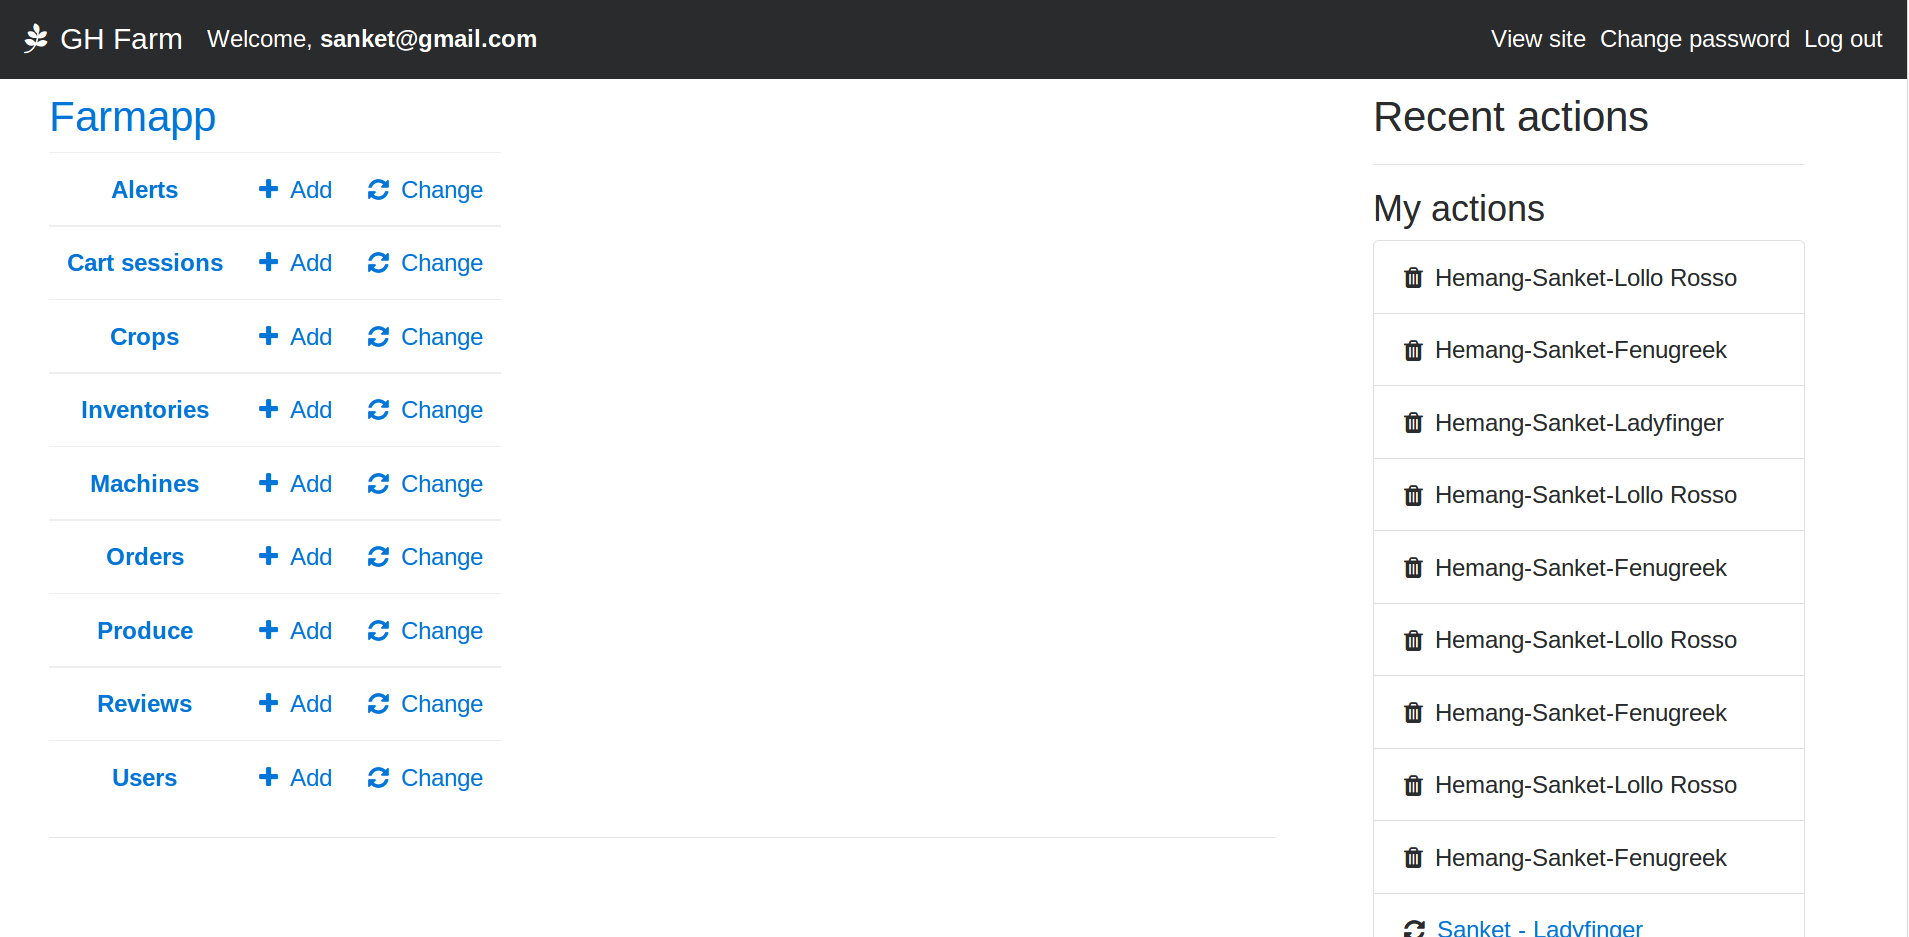
\includegraphics[width=1.0\linewidth]{admin.png}
		\end{figure}
		
		\subsubsection{Consumer Interface:}
		Consumers are the end users of the entire system. They can register onto the system and can buy the produce from the system and also rate the producers.
		\begin{figure}[!ht]
			\centering
			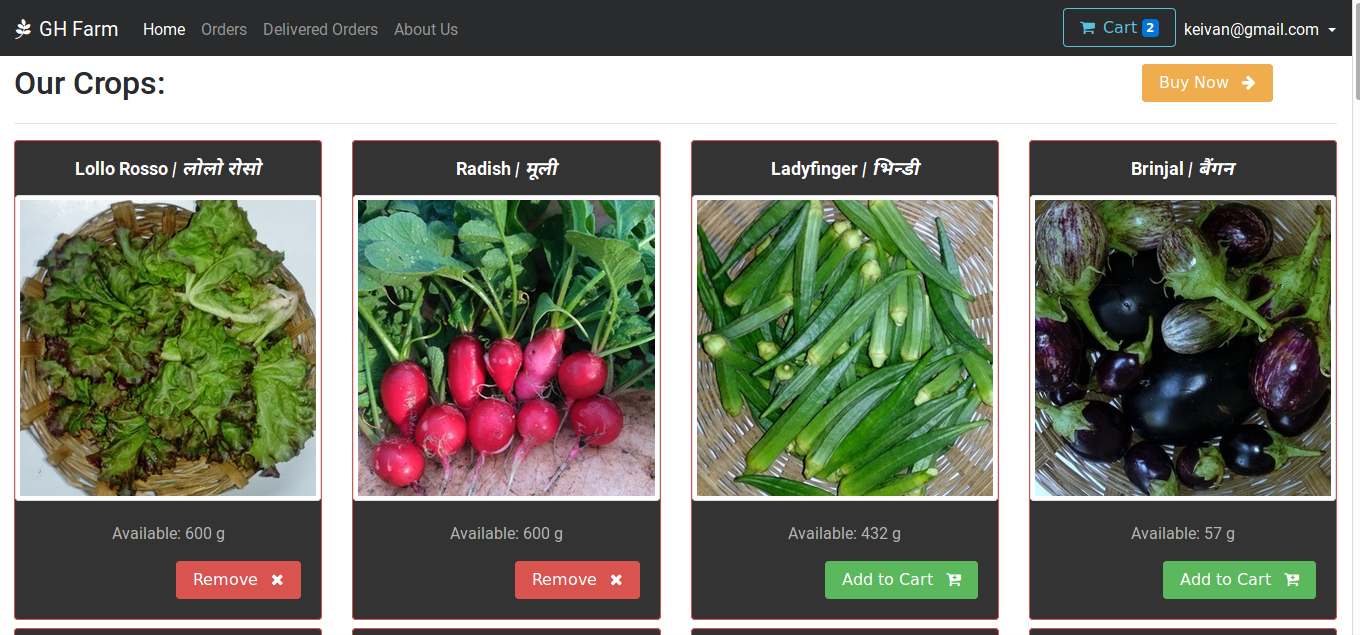
\includegraphics[width=1.0\linewidth]{screenshot.jpg}
		\end{figure}
		\newpage
		\subsubsection{Producer Interface:}
		Producers are the users who own the smart weighing machine and use them to add their produce to the system for monitoring and also to sell them. Each producer can have multiple machines allotted to him and all produce by this machines is logged into his account.
		\begin{figure}[!ht]
			\centering
			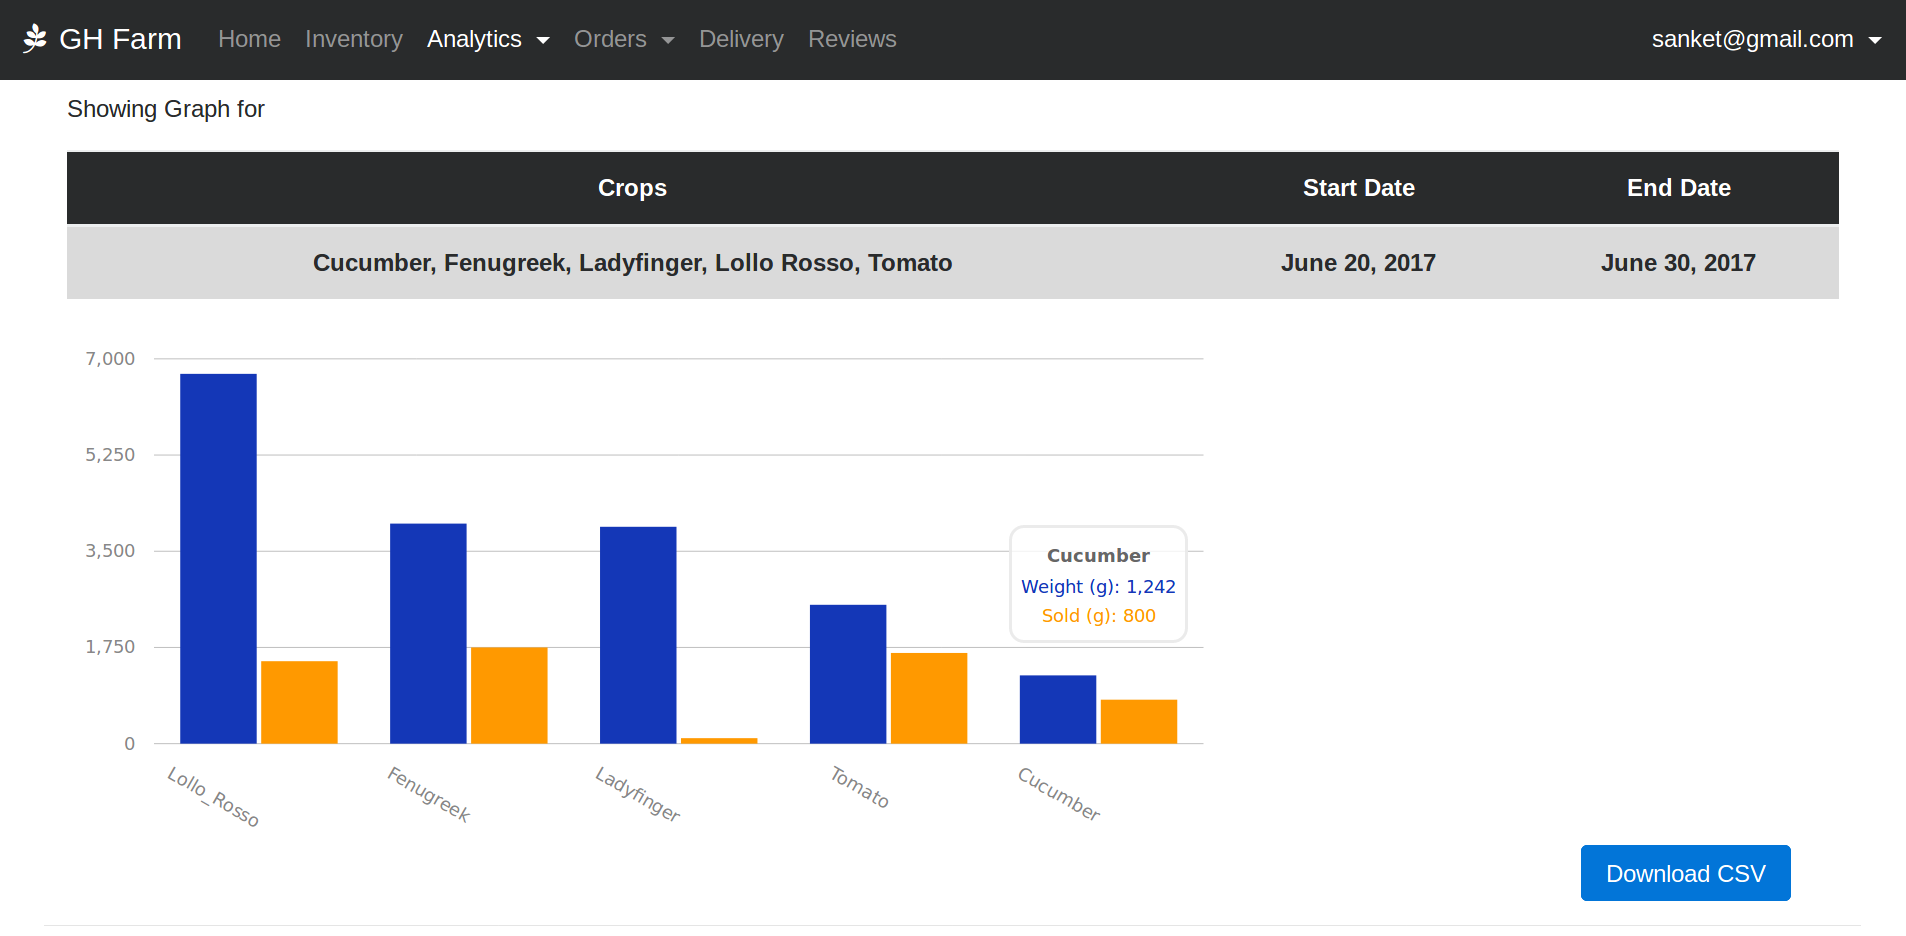
\includegraphics[width=1.0\linewidth]{analytics.png}
		\end{figure}
		
		Instructions to use the website can be obtained in our \href{https://github.com/eYSIP-2017/eYSIP-2017_Development_of_Web_Interface_for_GH_Farm_Produce/wiki}{wiki}.\\
		Visit the website : \href{http://store.k-yantra.org}{store.k-yantra.org}.\\
		
		
		\section{Future Work}
		\begin{enumerate}
			\item  \textbf{Include bill payment options:}\\
			Currently the website does not include a billing system which could be added in future.
			
			\item \textbf{Improve design of web interface:}\\
			The current UI is simplistic. It can be made more user friendly by improving the design.
		\end{enumerate}
		
		\section{Challenges Faced}
		\begin{enumerate}
			\item  \textbf{Handling Race Condition:}\\
			When a number of users concurrently access and modify the database it might leave the database in an inconsistent state. In order to avoid this situation we made use of transactions to maintain atomicity and made use of lock based protocol to establish concurrency control between the transactions.In lock based protocol, at a given time only one transaction can modify a table cell. This ensures consistency of the database. 
			
			\item \textbf{Caching:}\\
			One of a problem which we had never seen before was caching. The problem was that whenever the user filled up a form and was directed to a new page he can return to the filled up form by going back on the browser even tough the server code did not allow it. This was because of local caching by the browser. We later found a solution to this problem by including do not cache headers into HTTP response from the server.
			
			\item \textbf{Offline storage of data on raspberry pi:}\\
			There may occur a situation in which data sent by the smart weighing machine to the server is not sent properly due to no internet connectivity or some other errors.\\
			In such a situation data loss would occur. Thus the server sends an acknowledgement when it receives data from the smart weighing machine. In case of a failure to send data the machine would not receive appropriate acknowledgement and would store the data offline and try again later. This ensures that no data loss takes place.
			
		\end{enumerate}
		
		\begin{thebibliography}{li}
			\bibitem{}
			Django Documentation :
			{\href{https://docs.djangoproject.com/en/1.11/}{https://docs.djangoproject.com/en/1.11/}},
			\bibitem{}
			Djangogirls Tutorial :
			{\href{https://tutorial.djangogirls.org/en/}{https://tutorial.djangogirls.org/en/}},
			\bibitem{}
			Bootstrap 4 :
			{\href{https://v4-alpha.getbootstrap.com/}{https://v4-alpha.getbootstrap.com/}}
		\end{thebibliography}
		
		
	\end{document}